\chapter{Результаты}

Все численные методы были реализован в виде программ на языке C++ с использованием библиотеки CUDA \cite{cuda2015} для организации вычислений на графических процессорах. Использовались трехмерные сетки, сгенерированные программой NETGEN v4.9.14 \cite{Netgen2009}.
Для визуализации результатов применялась программа ParaView \cite{Paraview2004}.

\section{Исследование сходимости метода, основанного на вариационном принципе}

Исследование скорости сходимости проводились на задаче о плотности энергии излучения оптически плотного излучающего шара радиуса $R = 0.3$ в поглощающей оптически менее плотной среде (см. приложение \ref{sec:sphere}). В окрестности поверхности шара плотность энергии имеет логарифмическую особенность производной, такую же, как и в задаче Милна (задача об излучении из полупространства, см. приложение \ref{sec:milne}).

Изучалась ошибка в точках $A(0, 0, 0)$ --- центре шара, $B\left(\frac{R}{\sqrt{3}}, \frac{R}{\sqrt{3}}, \frac{R}{\sqrt{3}}\right)$ --- точке на границе шара в дискретной норме $L_2$:
\[
||u||_{DL_2} = \sqrt{\frac{1}{N}\sum_{i=1}^N u_i^2}
\]

Использовались пространственные сетки с количеством узлов от $7 \cdot 10^3$ до $206 \cdot 10^3$. Для метода сферических гармоник применялись сферические функции до $12$-й степени. Для метода радиальных базисных функций использовались $7$ первых квадратурных формул Лебедева в качестве сетки направлений. 

\subsection{Сходимость методов по количеству угловых функций}

Анализ сходимости в дискретной норме $L_2$ показал, что зависимость ошибки на самой подробной сетке ($206 \cdot 10^3$ узлов) от числа используемых угловых функций $K$ носит одинаковый характер $\varepsilon \sim K^{-0.29}$, причем ошибка обоих методов практически одинакова при одинаковом количестве используемых угловых функций, см. график на рисунке \ref{fig:UL2err}.

\begin{figure}[ht!]
\centering
\includegraphics[width=\textwidth]{UL2err.eps}
\caption{Ошибка в норме $||\cdot||_{DL_2}$ в зависимости от числа угловых функций $K$}
\label{fig:UL2err}
\end{figure}

\subsection{Пространственная сходимость методов}

Сходимость методов изучалась в точке $A$ из области гладкости и в точке $B$ на границе шара при использовании самой подробной угловой дискретизации. Сходимость изучалась в зависимости от характерного шага пространственной сетки, принятого равным $N^{-1/3}$. На рисунке \ref{fig:UAerr} изображены графики ошибки в области гладкости и на границе шара.

\begin{figure}[ht!]
\centering
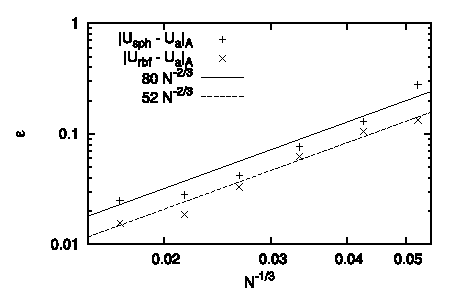
\includegraphics[width=.49\textwidth]{UAerr.eps}
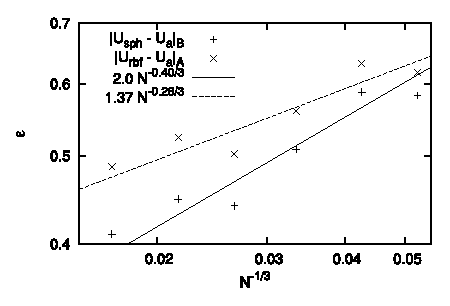
\includegraphics[width=.49\textwidth]{UBerr.eps}
\caption{Ошибка в точках $A, B$ в зависимости от характерного шага сетки $N^{-1/3}$}
\label{fig:UAerr}
\end{figure}

Порядок сходимости обоих методов в области гладкости равен двум. В области шара, где коэффициент поглощения меняется скачкообразно, порядок сходимости разный, он равен $\sim 0.4$ для метода сферических гармоник и $\sim 0.3$ для метода с радиальными базисными функциями, хотя разброс данных не позволяет достоверно определить порядок сходимости.

На рисунке \ref{fig:anvsnum} представлено решения вдоль оси $Ox$, полученные методом с радиальными функциями при $K = 55$ и методом сферических гармоник при $K = 91$. Видно, что существенное отличие численного решения от аналитического наблюдается в поглощающей области в окрестности шара.

Для обоих методов свойственны нефизичные значения интенсивности в области вдали от шара. Функция интенсивности, восстановленная из гармоник решения
\[
I(\vec r, \vec \Omega) = \sum_{k=1}^{n} I_k(\vec r) \theta_k (\vec \Omega)
\]
может содержать значения с отрицательными значениями интенсивности. В случае $I(\vec r, \vec \Omega) > 0$ тензор направленности излучения (тензор квазидиффузии) $\mathbb D$, определяемый как
\[
\mathbb D = \frac{\mathbb T}{U} = \frac{\int_{4\pi} \vec \Omega\vec \Omega I(\vec r, \vec \Omega) d\Omega}{\int_{4\pi} I(\vec r, \vec \Omega) d\Omega}
\]
имеет след, равный $1$ и неотрицательные компоненты. Однако, в численных расчетах свойство неотрицательности может нарушаться, если интенсивность $I(\vec r, \vec \Omega)$ принимает отрицательные значения (см. график на рисунке \ref{fig:Drad}). Значения $D_{rr} > 1$ свидетельствуют об отрицательности двух других главных компонент тензора $\mathbb D$.

\begin{figure}[ht!]
\centering
\includegraphics[width=.5\textwidth]{Uanvsnum.png}
\caption{Решения вдоль оси $Ox$, полученные методом с радиальными функциями при $K=55$ и методом сферических гармоник при $K = 91$}
\label{fig:anvsnum}
\end{figure}

\begin{figure}[ht!]
\centering
\includegraphics[width=.5\textwidth]{Dxx.png}
\caption{Радиальная компонента тензора направленноcти $\mathbb D_{rr}$ вдоль оси $Ox$}
\label{fig:Drad}
\end{figure}

Для исследования эффекта луча рассмотрим изоповерхности плотности интенсивности. Для метода сферических гармоник эффект луча отсутствует, поскольку базис из сферических функций инвариантен относительно произвольных вращений. На рисунке \ref{fig:iso} изображены изоповерхности решений, построенные для случая $K = 15$ метода сферических гармоник и $K = 13$ метода с радиальными функциями.

\begin{figure}[ht!]
\centering
\includegraphics[width=\textwidth]{iso.png}
\caption{Изоповерхности плотности энергии излучения для метода с радиальными функциями (слева) и сферическими гармониками (справа)}
\label{fig:iso}
\end{figure}

\subsection{Сходимость метода при использовании предобуславливателя}

Для исследования сходимости внешних итераций метода сопряженных градиентов изучалось количество вызовов предобуславливателя, необходимых для уменьшения нормы невязки в $10^{6}$ раз.

Отметим, что для метода сопряженных градиентов число итераций увеличивается как с увеличением количества угловых гармоник $K$, так и увеличением количества узлов сетки $N$. Для метода с радиальным базисом число итераций практически постоянно и равно $30$.

\begin{table}[ht!]
\RawFloats
\centering
\caption{Количество итераций метода сопряженных градиентов}
\begin{tabular}{cc|c|c|c|c|c|c|}
\cline{3-8}
& & \multicolumn{6}{|c|}{\rule{0em}{2.2ex}Количество узлов сетки} \\ \cline{3-8}
& & \rule{0em}{2.2ex}6996 & 12971 & 26786 & 53109 & 99015 & 205756\\ \cline{1-8}
\multicolumn{1}{|c|}{\multirow{7}{*}{\rotatebox{90}{Угловых  гармоник\phantom{x}}}} &
\multicolumn{1}{|c|}{\rule{0em}{2.2ex}1}  & 1 & 1 & 1 & 1 & 1 & 1 \\ 
\cline{2-8}\multicolumn{1}{|c|}{} &
\multicolumn{1}{|c|}{\rule{0em}{2.2ex}6}  & 20 & 21 & 22 & 23 & 25 & 26 \\ 
\cline{2-8}\multicolumn{1}{|c|}{} &
\multicolumn{1}{|c|}{\rule{0em}{2.2ex}15} & 29 & 31 & 33 & 34 & 37 & 38 \\ 
\cline{2-8}\multicolumn{1}{|c|}{} &
\multicolumn{1}{|c|}{\rule{0em}{2.2ex}28} & 36 & 38 & 41 & 44 & 48 & 51 \\ 
\cline{2-8}\multicolumn{1}{|c|}{} &
\multicolumn{1}{|c|}{\rule{0em}{2.2ex}45} & 42 & 45 & 49 & 53 & 57 & 62 \\ 
\cline{2-8}\multicolumn{1}{|c|}{} &
\multicolumn{1}{|c|}{\rule{0em}{2.2ex}66} & 46 & 50 & 55 & 60 & 65 & 70 \\ 
\cline{2-8}\multicolumn{1}{|c|}{} &
\multicolumn{1}{|c|}{\rule{0em}{2.2ex}91} & 48 & 53 & 59 & 65 & 71 & 77 \\ 
\cline{1-8}
\end{tabular}
\end{table}

\begin{table}[ht!]
\RawFloats
\centering
\caption{Количество итераций метода с радиальным базисом}
\begin{tabular}{cc|c|c|c|c|c|c|}
\cline{3-8}
& & \multicolumn{6}{|c|}{\rule{0em}{2.2ex}Количество узлов сетки} \\ \cline{3-8}
& & \rule{0em}{2.2ex}6996 & 12971 & 26786 & 53109 & 99015 & 205756\\ \cline{1-8}
\multicolumn{1}{|c|}{\multirow{7}{*}{\rotatebox{90}{Угловых гармоник\phantom{x}}}} &
\multicolumn{1}{|c|}{\rule{0em}{2.2ex}3}  & 13 & 14 & 15 & 14 & 15 & 15 \\ 
\cline{2-8}\multicolumn{1}{|c|}{} &
\multicolumn{1}{|c|}{\rule{0em}{2.2ex}7}  & 26 & 27 & 28 & 28 & 29 & 31 \\ 
\cline{2-8}\multicolumn{1}{|c|}{} &
\multicolumn{1}{|c|}{\rule{0em}{2.2ex}13} & 33 & 34 & 35 & 36 & 39 & 42 \\ 
\cline{2-8}\multicolumn{1}{|c|}{} &
\multicolumn{1}{|c|}{\rule{0em}{2.2ex}19} & 26 & 28 & 29 & 29 & 30 & 32 \\ 
\cline{2-8}\multicolumn{1}{|c|}{} &
\multicolumn{1}{|c|}{\rule{0em}{2.2ex}25} & 28 & 29 & 32 & 30 & 32 & 34 \\ 
\cline{2-8}\multicolumn{1}{|c|}{} &
\multicolumn{1}{|c|}{\rule{0em}{2.2ex}43} & 28 & 30 & 32 & 31 & 33 & 34 \\ 
\cline{2-8}\multicolumn{1}{|c|}{} &
\multicolumn{1}{|c|}{\rule{0em}{2.2ex}55} & 27 & 28 & 30 & 29 & 30 & 32 \\ 
\cline{1-8}
\end{tabular}
\end{table}

\section{Исследование маршевого метода коротких характеристик}

Для метода коротких характеристик изучалась численная диффузия луча. Центральное излучательное тело было заменено на крест, составленный из пяти одинаковых кубов (см. рисунок \ref{fig:cross}). Уравнение переноса решалось в одном направлении, при этом аналитическое решение представляет собой проекцию креста на грань тетраэдра. Оптическая толщина излучающего тела много больше единицы, а оптическая толщина окружающего пространства много меньше единицы. В таких условиях, решение на грани имеет интенсивность равную равновесной интенсивности в кресте.
\begin{figure}[ht!]
\centering
\includegraphics[width=.5\textwidth]{plus.png}
\caption{Вид излучающего тела для метода коротких характеристик}
\label{fig:cross}
\end{figure}

%\subsection{Сравнение численной диффузии луча в методах первого и второго порядка}

Для метода первого порядка решение на грани испытывает значительную диффузию. Для метода второго порядка без ограничителя решение нарушает принцип максимума. Отклонения интенсивности на грани от диапазона $[0, 1]$ составляет $20 \%$ (области на границе креста). Метод с ограничителем имеет решение, в котором принцип максимума не нарушен, а численная диффузия луча значительно меньше, чем в случае метода первого порядка.

\begin{figure}[ht!]
\centering
\includegraphics[width=.3\textwidth]{res1ord.png}
\includegraphics[width=.3\textwidth]{res2nolim.png}
\includegraphics[width=.3\textwidth]{res2wilim.png}
\caption{Решение на грани для метода первого порядка (слева), метода второго порядка (в центре) и метода второго порядка с ограничителем (справа)}
\label{fig:limiter}
\end{figure}

Сравнение плотности излучения в решениях, полученных методом первого и второго порядка с ограничителем, показывает близкие (в пределах $2\%$) решения (см. графики на рисунках \ref{fig:U2vs1} и \ref{fig:U2vs1Line}). При этом для метода второго порядка плотность энергии излучения сосредоточена в кресте, в то время как в методе первого порядка она диффундирует за его пределы. К тому же, в методе второго порядка более выражен эффект луча, в методе же первого порядка он сглажен численной диффузией.

\begin{figure}[ht!]
\centering
\includegraphics[height=.35\textheight]{U2vs1.png}
\caption{Плотность излучения в методе первого порядка (слева) и второго порядка с ограничителем (справа) в центральном сечении}
\label{fig:U2vs1}
\end{figure}

\begin{figure}[ht!]
\centering
\includegraphics[height=.35\textheight]{U2vs1Line.png}
\caption{Плотность излучения в методе первого порядка (синий график) и второго порядка с ограничителем (красный график) вдоль луча, перпендикулярного кресту}
\label{fig:U2vs1Line}
\end{figure}

Дополнительно был рассмотрен метод первого порядка с увеличенным количеством узлов. В этом методе вместо квадратичной интерполяции по шести узлам используется кусочно-линейная. Данная операция позволяет сравнивать методы при одинаковом числе используемых узлов. 

Рассматривалась задача об излучении шара в сферической области. Поглощение в области отсутствовало. Диффузия луча носит качественно различный характер: в методе первого порядка диффузия луча имеет характер $\sim \sqrt{x}$, а в методе второго порядка диффузия луча постоянна вдоль луча, см. график на рисунке \ref{fig:diffus}.

\begin{figure}[ht!]
\centering
\includegraphics[width=\textwidth]{diff.png}
\caption{Диффузия луча в методе первого порядка с увеличенным числом узлов (слева) и методе второго порядка с ограничителем (справа)}
\label{fig:diffus}
\end{figure}

\section{Исследование распределенного метода длинных характеристик}

Данный метод тестировался на той же модельной задаче, что и метод, основанный на вариационном принципе. Использовалась пространственная сетка с $66 \cdot 10^{3}$ узлов ($363 \cdot 10^{3}$ тетраэдров) и угловая сетка из $230$ направлений (квадратурная формула Лебедева $25$-го порядка). Область разбивалась на $2, 3, 4$ и $8$ подобластей с помощью библиотеки METIS \cite{METIS}.  Для решения разреженной системы линейных уравнений применялась библиотека UMFPACK \cite{umfpack2004}. Для организации распределенных вычислений использовалась библиотека OpenMPI \cite{MPI}.

\subsection{Сравнение решений для различного числа подобластей}

В случае нескольких подобластей метод имеет незначительную диффузию луча, проходящего через поверхность раздела подобластей.
На рисунке \ref{fig:diff} приведены решения для случая одной подобласти и восьми подобластей. Численная диффузия в данном методе несоизмеримо меньше численной диффузии в методе коротких характеристик.
На рисунке \ref{fig:split} можно видеть разбиение области на подобласти (показаны 4 из 8).

\begin{figure}[ht!]
\includegraphics[width=.35\textwidth]{res1piece}
\includegraphics[width=.35\textwidth]{res8pieces}
\caption{Срез решения в одном направлении. Слева одна подобласть, справа --- 8}
\label{fig:diff}
\end{figure}

\begin{figure}[ht!]
\centering
\includegraphics[width=.35\textwidth]{ressplit.png}
\caption{Используемая декомпозиция области на подобласти}
\label{fig:split}
\end{figure}

Если пренебречь численной диффузией, метод имеет эталонную точность для каждого направления. Однако, это приводит к наиболее выраженному эффекту луча среди всех исследованных методов, см. изоповерхности решения на рисунке \ref{fig:isomcm}. Наиболее выражены искажения вдоль координатных осей $Ox, Oy, Oz$. В этих направлениях веса квадратурной формулы Лебедева максимальны.

\begin{figure}[ht!]
\centering
\includegraphics[width=.4\textwidth]{isomcm.png}
\caption{Изоповерхности плотности излучения, полученной распределенным методом длинных характеристик}
\label{fig:isomcm}
\end{figure}

\subsection{Ускорение и эффективность параллельной реализации}

В таблице \ref{tab:speedup} приведено сравнение времени работы алгоритма при различных разбиениях расчетной области. Данные результаты получены на высокопроизводительном стенде кафедры информатики и вычислительной математики МФТИ. Незначительное ускорение обусловлено хаотическим доступом к памяти при трассировке лучей, плохой балансировкой нагрузки на графическом ускорителе, а также значительным количеством условных операторов в коде трассировки. 
\begin{table}[ht!]
\RawFloats
\centering
\caption{Время работы алгоритма в зависимости от числа подобластей $P$ для MPI-реализации (CPU) и MPI+CUDA-реализации (GPU)}
\begin{tabular}{|c|c|c|c|c|}
\hline
$P$ & Устройства & $t_\text{GPU}, \text{c}$ & $t_\text{CPU}, \text{c}$ & $t_\text{CPU} / t_\text{GPU}$\\\hline
$1$& 1 $\times$ Tesla C2075 & $117$ & $439$ & $3.75$x\\\hline
$2$& 2 $\times$ Tesla C2075 & $52$ & $196$ & $3.77$x\\\hline
$3$& 3 $\times$ Tesla C2075 & $32.7$ & $125$ & $3.82$x\\\hline
$4$& 3 $\times$ Tesla C2075 + GTX 680 & $28.1$ & $108$ & $3.84$x\\
%    $4$& 1 x Tesla C2075 & $88$ & $108$ & $1,23$x\\
\hline
$8$& 3 $\times$ Tesla C2075 + GTX 680 & $25.5$ & $69$ & $2.70$x\\\hline
\end{tabular}
\label{tab:speedup}
\end{table}

Отметим сверхлинейное ускорение как CPU, так и GPU версии программы. Оно вызвано тем, что распределенный метод не является параллельной версией метода длинных характеристик, а является другим параллельным методом, решение которого зависит от числа подобластей и способа разбиения. Если не принимать во внимание это обстоятельство, эффективность распараллеливания
\[
E_P = \frac{S_P}{P}, \quad S = \frac{t_1}{t_P}
\]
достигает $120 \%$ при $P = 3$. Сверхлинейное ускорение вызвано уменьшением средней длины характеристики при разбиении области на подобласти. Учитывая, что при разбиении на $3$ подобласти средняя длина характеристики сокращается в $\sqrt[3]{3} \approx 1.44$ раз, реальная эффективность распараллеливания составляет 
\[
\tilde E_P = \frac{E_P}{\sqrt[3]{P}}.
\]
Для $P=2$ эта величина равна $\tilde E = \frac{117}{2 \cdot 52 \sqrt[3]{2}} \approx 89 \%$, а для $P = 3$ --- $\tilde E_3 = \frac{117 \%}{3 \cdot 32.7\sqrt[3]{3}} \approx 83 \%$. Аналогичные показатели для реализации с графическими ускорителями отличаются незначительно.

\section{Расчет спектра излучения линии H-$\alpha$ звезды типа Т Тельца}

Для численного воспроизведения спектра излучения линии H-$\alpha$ были использованы поля гидродинамических величин из работы \cite{romanova2009}. В этой работе с помощью математического моделирования изучалось взаимодействие звезды с ее аккреционным диском. Магнитный момент звезды составлял угол в $30^\circ$ к направлению вращения звезды, что при определенных условиях падения вещества на звезду приводило к образованию конического ветра (см. рисунок \ref{fig:wind}).
\begin{figure}[ht!]
\centering
\includegraphics[width=.4\textwidth]{wind.png}
\caption{Изоповерхность плотности вещества, окружающего звезду. Цвет соответствует величине радиальной компоненты скорости}
\label{fig:wind}
\end{figure}

В работе \cite{romanova2009} расчет проводится в безразмерных единицах, а результаты могут быть применены к широкому набору астрофизических задач подстановкой конкретных размерных единиц, при условии сохранения тех же безразмерных определяющих параметров. Значения размерных единиц были подставлены для случая классической звезды Т Тельца. Также, был проведен расчет с увеличенным значением единицы измерения магнитного поля $B_0 = 40 \text{ Гс}$ вместо $B_0 = 12.5 \text{ Гс}$, что соответствует увеличению единицы измерения плотности в $10$ раз, без изменения характерного масштаба длины. 

В работе \cite{romanova2009} приняты следующие размерные единицы: 
\begin{itemize}
\item единица измерения длины $R_0 = 2 R_*$, где $R_*$ --- радиус звезды;
\item единица измерения массы $M_0 = M_*$, где $M_*$ --- масса звезды;
\item единица измерения скорости $v_0 = \sqrt\frac{GM}{R_0}$ --- единица скорости;
\item единица измерения магнитного поля $B_0 = \frac{B_*}{\bar \mu} \left(\frac{R_*}{R_0}\right)^3$, где $B_*$ --- магнитное поле на поверхности звезды, $\bar \mu$ --- безразмерный магнитный момент звезды;
\item единица измерения температуры $T_0 = \frac{v_0^2}{\mathcal R}$, где $\mathcal R$ --- универсальная газовая постоянная;
\item единица измерения плотности $\rho_0 = \frac{B_0^2}{v_0^2}$
\item единица измерения давления $p_0 = B_0^2 = \frac{\rho_0}{\mathcal{R} T_0}$.
\end{itemize}

Подставляя безразмерные единицы в формулы для коэффициента поглощения \eqref{eq:absorb}, получаем 
\[
R_0 \varkappa_\nu(v_0 \Delta \tilde v) = \frac{\varkappa \lambda_0 R_0}{v_0} \frac{1}{\sqrt{2\pi \tilde T}} \exp\left(
-\frac{(\Delta  \tilde v + \tilde {\vec v} \vec k)^2}{2\tilde T}
\right),
\]
где величины с тильдой являются обезразмеренными.

В качестве расчетной области использовалась полусфера, увеличенная так, чтобы содержать центральное излучающее тело --- звезду. Расчетная сетка состояла из $713 \cdot 10^3$ узлов ($4 \cdot 10^6$ тетраэдров). Расчет проводился распределенным методом длинных характеристик.
Использовалась равномерная по полярному углу сетка направлений. Для каждого значения полярного угла
азимутальная сетка строилась так, чтобы расстояние между соседними направлениями было приблизительно одинаковым. Угловая сетка содержала $1091$ направление. Такая сетка позволила получить усредненные по периоду обращения звезды спектры при различных углах наклонения $i$ (угол между плоскостью диска и лучом зрения). Использовалось $64$ частотные группы в интервале, соответствующем доплеровскому смещению линии H-$\alpha$ от $-600 \text{ км}/\text{c}$ до $600 \text{ км}/\text{c}$. Для каждого направления $\vec \omega_i$ вычислялся интегральный поток излучения, уходящего с поверхности шара в направлении $\vec \omega_i$. Также, благодаря использованию распределенного метода длинных характеристик, стало возможным отключить блок трассировки внутренности подобластей, что значительно сократило время вычислений. Для расчетов использовались два узла кластера лаборатории флюидодинамики и сейсмоакустики МФТИ, на каждом узле использовалось 8 графических ускорителей. На данной задаче было достигнуто ускорение $4.5$ раза по отношению к MPI-реализации без использования графических ускорителей.

Зависимость усредненной за период обращения звезды относительной интенсивности $I_\text{o}$ от частоты излучения при разных углах наклонения $i$ представлена на рисунке \ref{fig:spectre}. Для удобства смещение частоты $\Delta \nu$ переведено в относительную скорость $\Delta v = c \frac{\Delta \nu}{\nu_0}$. Можно заключить, что при углах наклонения $i \lesssim 45^\circ$ поглощение в диапазоне синего смещения $\Delta v \sim 150 \dividesymbol 200 \text{ км}/\text{с}$ существенно лишь для случая $B_0 = 40 \text{ Гс}$. Нормализованный профиль линии излучения имеет существенный провал в области красного смещения на скорости $\Delta v \approx 100 \text{ км}/\text{с}$, который объясняется значительным поглощением излучения веществом диска, аккрецирующего на звезду. Для случая $B_0 = 12.5 \text{ Гс}$ существенное поглощение в линии спектра наблюдается лишь для направлений, близких к плоскости диска. 
\begin{figure}[ht!]
\centering
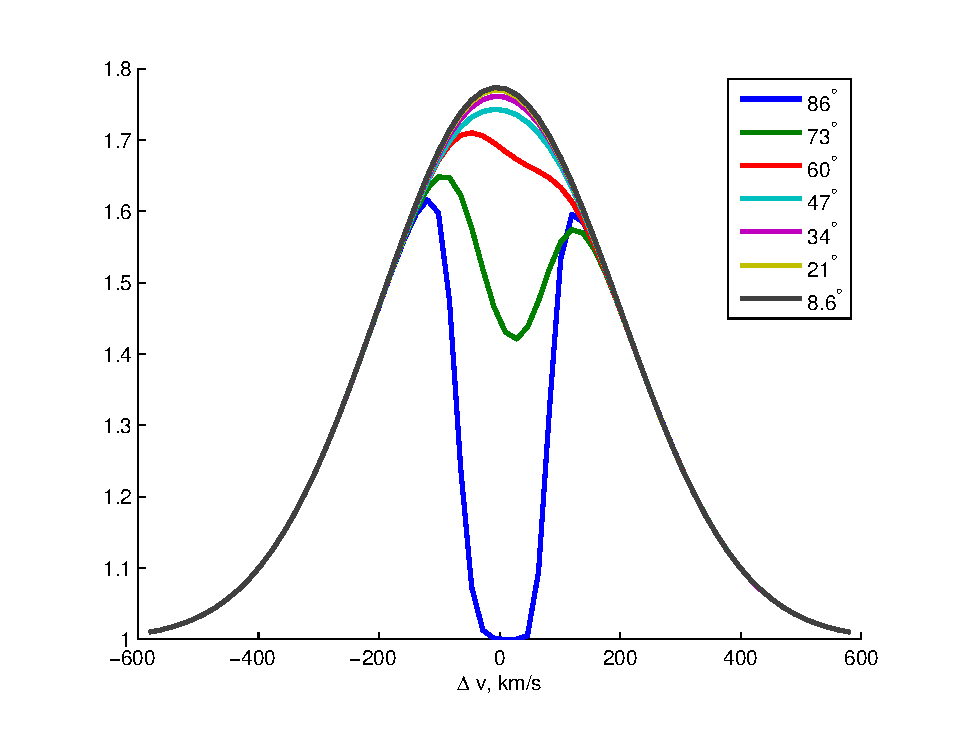
\includegraphics[width=.6\textwidth]{spectrum-bad.eps}
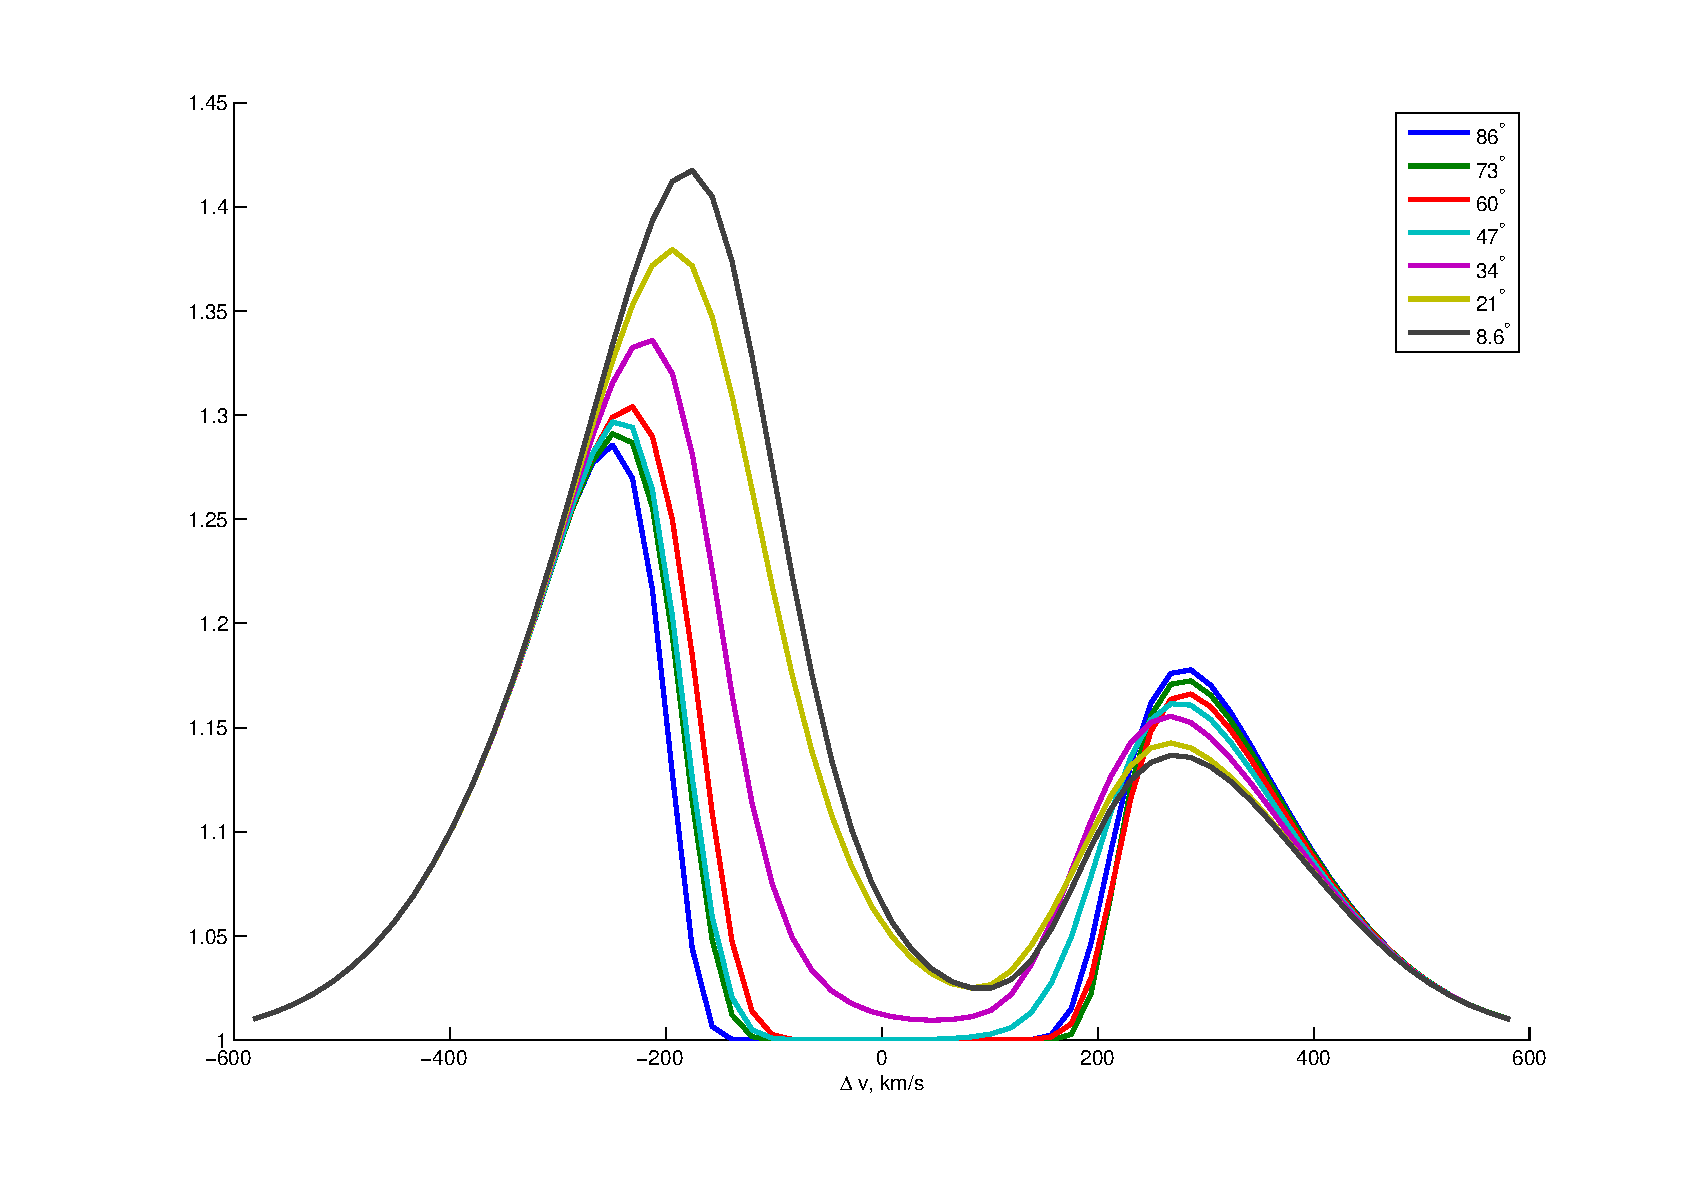
\includegraphics[width=.6\textwidth]{spectrum.eps}
\caption{Профиль линии H-$\alpha$ в зависимости от угла наклонения $i$ для случая $B_0 = 12.5 \text{ Гс}$ (сверху) и $B_0 = 40 \text{ Гс}$ (снизу)}
\label{fig:spectre}
\end{figure}

\FloatBarrier

\section{Выводы}

Основанные на вариационном принципе методы (метод сферических гармоник и метод с радиальным базисом)  демонстрируют сходное поведение: оба метода сходятся со вторым порядком в области гладкости и с порядком, меньшим единицы, в области особенности градиента решения. Ошибка в дискретной норме $L_2$ не зависит от типа угловой дискретизации, а зависит лишь от количества угловых функций $K$. Метод с радиальными базисными функциями сходится за меньшее количество вызовов предобуславливателя, но не обладает свойством инвариантности относительно поворотов, то есть имеет выделенные направления.

Для метода коротких характеристик второго порядка осцилляции могут составлять до $20\%$. Использование ограничителя полностью их устраняет. В методе второго порядка сильнее выражен эффект луча, в то время, как в методе первого порядка, он сглажен из-за численной диффузии. Точность метода второго порядка обусловлена не только повышенным числом узлов, так как метод второго порядка оказался более точным по сравнению с методом, использующим кусочно-линейную интерполяцию по шести точкам.

Распределенный метод длинных характеристик обладает высокой точностью метода длинных характеристик. Решения, полученные данным методом, имеют незначительную диффузию луча, проходящего через границу раздела подобластей. Эффект луча в данном методе выражен наиболее сильно. Реализация метода с использованием графических ускорителей показала ускорение примерно в $4$ раза относительно MPI-версии. Такое незначительное ускорение может быть объяснено случайным доступом к памяти и плохой балансировкой загрузки нитей.

Проведено численное моделирование формы линии H-$\alpha$ в спектре звезды Т Тельца из работы \cite{romanova2009}. Показано, что  поглощение наблюдается не только в области синего смещения, но и в области красного смещения. Поглощение в области красного смещения вызвано веществом, аккрецирующем на звезду.
